%%%%%%%%%%%%%%%%%%%%%%%%%%%%%%%%%%%%%%%%%%%%%%%%%%%%%%%%%%%%%%%%%%%%%%%%%%%
%
% Plantilla para un artículo en LaTeX en español.
%
%%%%%%%%%%%%%%%%%%%%%%%%%%%%%%%%%%%%%%%%%%%%%%%%%%%%%%%%%%%%%%%%%%%%%%%%%%%

% Qué tipo de documento estamos por comenzar:
\documentclass[12pt]{article}
\usepackage{graphicx}
\usepackage{multicol}
\newcommand\tab[1][1cm]{\hspace*{#1}}


\title{Plantilla para un artículo \LaTeX}
\author{
  Domínguez-Adame Ruiz, Alberto\\
  \small Universidad de Sevilla\\
  \small albdomrui@alum.us.es\\
  \small Sevilla
  \date{}
  \and
 Vilaplana de Trias, Francisco David\\
  \small Universidad de Sevilla\\
  \small fravilde1i@alum.us.es\\
  \small Sevilla
  \date{}
}


%% Después del "preámbulo", podemos empezar el documento

\begin{document}
%% Hay que decirle que incluya el título en el documento


\maketitle




%% Aquí podemos añadir un resumen del trabajo (o del artículo en su caso) 
\begin{abstract}
Esta es una plantilla simple para crear un articulo \LaTeX en español, con algunos comandos que se usarán frecuentemente para hacer tareas de la licenciatura en Física.
\end{abstract}


%% Iniciamos "secciones" que servirán como subtítulos
%% Nota que hay otra manera de añadir acentos
\section{Introducci\'on}


\tab[0,65cm]Para empezar, el aprendizaje se define como la adquisición del conocimiento de algo por medio del estudio, el ejercicio o la experiencia, en especial de los conocimientos necesarios para aprender algún arte u oficio. Al hablar sobre el aprendizaje automático estaríamos entrando en el campo de la Inteligencia Artificial (IA). Podemos definir esta como un programa de computación diseñado para realizar determinadas operaciones que se consideran propias de la inteligencia humana, como el Aprendizaje Automático (Machine Learning), una rama de la inteligencia artificial, cuyo objetivo es el desarrollo de un sistema (modelo matemático que realiza una determinada tarea)  el cual tiene un mejor desempeño con la experiencia, dados una serie de datos.

Nuestro estudio hace uso de datos relacionales, los cuales están unidos entre sí (tienen una relación) que queda representado como aristas en un grafo, entendiendo un grafo como un conjunto de nodos unido (o no) mediante aristas. En la Figure \ref{fig:tablaEj} podemos ver un ejemplo de un grafo a partir de unos datos relacionales. 

Para la realización de este trabajo se ha hecho uso del entorno de desarrollo Jupyter y de la herramienta notebook. El código está escrito mediante el lenguaje de programación Python, usando principalmente las librerías pandas, NetworkX y scikit-learn, y otras como keras, tensorflow y matplot.


Los modelos de clasificación usados son: KNN, Naive Bayes, Árboles de Decisión y Redes Neuronales.


\section{Conjunto de datos y Tarea de predicción a realizar}
ddlknvdsankbndnbkndv

\section{Métricas Relacionales}
HOAL

\section{Algoritmos de Aprendizaje Automático}

\subsection{KNN}

Primero tienes que cargar el archivo de imagen desde su computadora usando el enlace de carga del menú del proyecto. Luego usando el comando 'includegraphics' podrás incluirlo en el documento. Con el entorno de figura y el comando de título podrás agregar un número y un título a la figura. Mira el código de la Figura \ref{fig:tablaEj} en esta sección para ver un ejemplo.


\begin{figure} % opción de posicionamiento
    \centering
    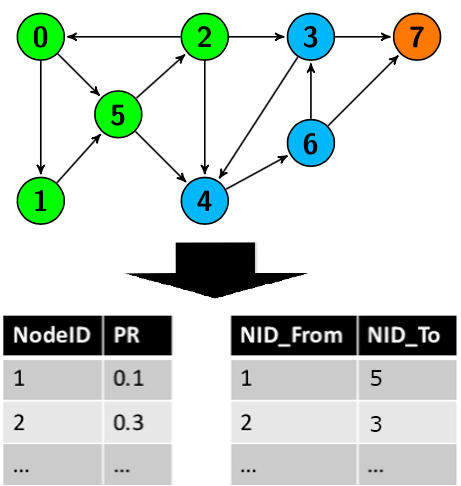
\includegraphics[width=0.5\textwidth]{./ImagenesMemoria/TablaEjemplo}
    \caption{\label{fig:tablaEj}Tabla de Ejemplo}
\end{figure}


\subsection{Naive Bayes}
% * <stephmigoni@gmail.com> 2018-02-08T19:23:33.559Z:
% 
% Esto es un comentario de prueba
% 
% 

Puedes añadir comentarios en el ícono + del menú de arriba.

Para responder a un comentario, simplemente da click en Reply en Rich Text.


También pueden añadirse comentarios en el margen del pdf compilado con el comando todo, como se muestra en el ejemplo de la derecha. También puedes añadirlos dentro del texto:

\subsection{Árboles de Decisión}

Usa los comandos table y tabular para iniciar una tabla simple --- mira la tabla~\ref{tab:tabla ejemplo}, como ejemplo. 

\begin{table}
\centering
\begin{tabular}{l c r} 
%nùmero de columnas: 3
l para left & c para centro & r para derecha \\ \hline
Ejemplo & Centrado & Alineado a la\\
Izquierda & 13 & Derecha
\end{tabular}
\caption{\label{tab:tabla ejemplo}Una simple tabla.}
\end{table}

\subsection{Redes Neuronales}

\LaTeX{} es buenísimo para escribir ecuaciones. Para escribir variables o ecuaciones dentro del texto lo podemos poner entre signos de pesos y luego podemos seguir escribiendo, esto funciona si queremos escribir un símbolo como $\nabla$, $\pi$, $\beta$, $\Omega$, $\aleph$, etc.
\begin{equation}
\sum_{n=0}^\infty \frac{x^n}{n!}=e^x
\end{equation}
\begin{equation}
\int_{0}^{1}dx=1
\end{equation}
\begin{equation}
e^{i\pi}+1=0
\end{equation}
Si queremos citar al gran Maxwell, lo podemos hacer como en la ecuación \ref{eq:Maxwell}:
\begin{equation}
\nabla\times\mathbf{E}+\frac{\partial\mathbf{B}}{\partial t}=0\label{eq:Maxwell}
\end{equation}

A continuación se añade un ejemplo de un desarrollo:
Con este preámbulo llevamos a cabo la siguiente transformación de los operadores $\hat{a}_{\ell}$

\begin{equation}
\hat{b}_{m}^{\dagger}=\sum_{\ell}U_{m}^{\ell}\hat{a}_{\ell}^{\dagger}
\end{equation}

donde $U_{m}^{\ell}$ es un elemento de la matriz unitaria $\mathbf{U}$.



\section{Resultados}

Puedes añadir listas con numeración automática \dots

\begin{enumerate}
\item Como esta,
\item y como esta.
\end{enumerate}
\dots o con puntitos \dots
\begin{itemize}
\item Como este,
\item y como este.
\end{itemize}



\section{Conclusiones}

\section{Bibliografía}



\end{document}